% !TEX program = xelatex
% !TEX encoding = UTF-8 Unicode
% main.tex  ——  CUMCM 2026 B题论文
\documentclass[12pt,a4paper]{ctexart}

% ===== 宏包 =====
\usepackage{amsmath,amssymb,amsthm}
\usepackage{geometry}
\usepackage{graphicx}
\usepackage{booktabs}
\usepackage{tabularx}
\usepackage{array}
\usepackage{multirow}
\usepackage[hidelinks]{hyperref}
\usepackage{xcolor}
\usepackage{caption}
\usepackage{subcaption}
\usepackage{float}
\usepackage{enumitem}
\usepackage{bm}
\usepackage{algorithm}
\usepackage{algorithmic}

% ===== 页面 =====
\geometry{left=2.5cm,right=2.5cm,top=2.5cm,bottom=2.5cm}
\setlength{\parindent}{2em}
\setlength{\parskip}{2pt}

% ===== 定理环境 =====
\newtheorem{theorem}{定理}[section]
\newtheorem{lemma}[theorem]{引理}
\newtheorem{corollary}[theorem]{推论}
\newtheorem{definition}{定义}[section]
\newtheorem{remark}{注}[section]

% ===== 算子与宏 =====
\DeclareMathOperator{\diam}{diam}
\DeclareMathOperator{\conv}{conv}
\newcommand{\R}{\mathbb{R}}
\newcommand{\eps}{\varepsilon}
\newcolumntype{C}{>{\centering\arraybackslash}X}
\newcolumntype{L}{>{\raggedright\arraybackslash}X}

% ===== 图路径（相对于 paper/ 目录）=====
\graphicspath{{./figures/}}

\begin{document}

%% ===== 摘要页 =====
\thispagestyle{plain}
\setcounter{page}{1}
\begin{center}
  {\LARGE\bfseries 无线电干扰源的快速自动定位与清除}\\[8pt]
  {\large 2026 年全国大学生数学建模竞赛 \, B 题}
\end{center}

\vspace{1em}
\noindent\textbf{摘\quad 要}

\vspace{0.5em}
在日益复杂的无线电频谱管理场景下，干扰源定位与清除直接关系到公共安全与应急效率。针对含测向误差、多源未知、定向未知等约束的干扰源自动定位清除问题，本文综合运用交会定位、计算几何、最小二乘定位及启发式搜索，建立了从单源交会定位到多源搜索清除的系统性优化模型，旨在为机器狗在危险环境中高效清除干扰源提供理论支撑与算法框架。

\textbf{对于问题一}，将示向度 $\pm1°$ 误差建模为以检测点为顶点、张角 $2°$ 的凸楔形，用两个半平面的交等价表示以规避方位角回绕；定位区域由全部楔形与目标圆域取交，采用 Sutherland--Hodgman 逐次半平面裁剪求顶点，再以旋转卡壳在 $O(h)$ 时间内计算凸多边形直径，并以顶点对暴力枚举互为校验，两者偏差不超过 $10^{-9}$ 米。Thales 逆定理给出覆盖的充要判据；以 Jung 定理证明最坏情况下最小覆盖圆直径比定位直径大不超过 $15.5\%$。24053 组随机构型的统计表明四个典型案例：正交 $\gamma=90°$ 时直径 62.86 m、偏侧 $\gamma=32.7°$ 时直径 192.61 m、三站等边时直径 57.05 m，三者直径圆均覆盖；而三站近等边、源近重心时最坏张角 $88.891°<90°$，直径圆失效，最小覆盖圆直径比定位直径大 $0.96\%$。随机采样低估最坏比值（采样最大值仅 $1.0008$），故给出"典型近似覆盖、最坏可达 $1.010$"的分层结论。

\textbf{对于问题二}，推导两方位线在角扰动下的交点位移公式；在垂直布站特例下得到完整闭式解：最优基线 $b^{*}=\sqrt{2}\,r$、最优交会角 $\alpha^{*}=\arccos(1/\sqrt{3})=54.74°$、最小定位误差 $E_{\min}=3\delta r=0.052360\,r$。针对目标距离未知的实情，以期望定位误差为目标函数做二维寻优：最优布站为基线 $1392.7\,\text{m}$、偏离示向度 $20.15°$，期望误差 $22.13\,\text{m}$；垂直布站在其最优基线 $1500\,\text{m}$ 处期望误差仍高达 $55.30\,\text{m}$（为最优方案的 $2.5$ 倍），且该劣势随基线加长并不改善，说明其根源在\emph{方向}而非\emph{长度}。候选区域为半径 $1240\sim1620\,\text{m}$、偏离示向度 $14°\sim29°$ 的对称圆弧带。

\textbf{对于问题三}，提出"全域粗探—交会定距—迭代逼近—就地清除"四阶段策略。粗探阶段取"中心加半径 $1122.96\,\text{m}$ 六边形环"七点覆盖网，该半径由闭式解 $r=(R\sqrt3-\sqrt{4R_c^2-R^2})/2$ 给出，恰使区域内最坏覆盖距离等于接收半径下界 $1000\,\text{m}$，50 m 步长采样 4053 点验证零遗漏。由问题二结论反解出清除精度所需逼近距离阈值为 $381.97\,\text{m}$。实测标定：本地 mock 35 局（源数 $8\sim16$ 各 7 种子）与官方模拟器演练 10 局全部零漏源，前者清除 $420/420$、$T$ 均值 $4601\,\text{s}$，后者清除 $129$ 个源、$T$ 均值 $4519\,\text{s}$、平均定位清除时间 $355.4\,\text{s}/\text{源}$；两环境在总量（偏差 $1.8\%$）与成本结构（移动占比 $80\%\sim85\%$）上互相印证。$1$ 次正式测试给出 $7874.47\,\text{s}$、$13$ 个源、单源 $605.7\,\text{s}/\text{源}$，暴露出内层七点共圆导致交会角仅 $15°\sim30°$ 的缺陷；改为"近圈 $400\,\text{m}$ 三点 $+$ 远圈 $1600\,\text{m}$ 四点"的混合内层后，$45$ 局演练的虚拟时间均值由 $6756\,\text{s}$ 降至 $4582\,\text{s}$（$-32.2\%$），单源耗时回归 $323.3\,\text{s}/\text{源}$。

\textbf{对于问题四}，证明"背向不可测定理"（视角差 $\geq180°$ 的两点不可能同时无信号），给出零漏测的方位包围充要判据；七点覆盖网对定向源的理论命中率约 $99.2\%$，对"全程无信号"频道采用加密补测策略。$50\%$ 定向源比例下的 35 局本地实测可清除 $386/420$ 个源，漏源率 $8.1\%$，代价为 $37.7\%$ 的额外虚拟时间；且漏源与源数无关、与定向源朝向的偶然性直接相关，为后续改进指明方向。$1$ 次正式测试给出 $7798.95\,\text{s}$、$16$ 个源、单源 $487.4\,\text{s}/\text{源}$，清除失败仅 $2$ 次，优于同期问题三——$25$ 点全覆盖网的采样密度足以支撑交会角，从反面印证了交会角对定位效率的主导作用。

\vspace{0.5em}
\noindent\textbf{关键词}：交会定位；旋转卡壳；Thales 判据；Jung 定理；误差传播；Kershner 覆盖；方位包围

\newpage
\tableofcontents
\newpage

% ===== 正文 =====
\section{问题重述与分析}
\label{sec:intro}

\subsection{问题背景}

机器狗在半径 $R=1800\,\text{m}$ 的圆形目标区域 $D$ 内搜索、定位并清除 $10\sim16$ 个无线电干扰源。每个干扰源占用频道 $1\sim20$ 中的唯一频道，有效接收半径 $r_c\in[1000,1500]\,\text{m}$（具体值未公开）。全向源在任意方向发射；定向源仅覆盖以其定向方向为中心、两侧各 $90°$ 的半圆锥体。机器狗在检测点通过 \texttt{/measure} 接口获取当前频道的\textbf{示向度}（干扰源相对于检测点的方位角，误差 $\pm1°$），通过 \texttt{/clear} 在距干扰源 $\leq20\,\text{m}$ 处实施清除，运行时间上限为 20 分钟。

\subsection{四个子问题的层次关系}

问题一、二属于纯几何推导，是算法设计的理论基础：问题一给出定位区域的精确刻画与直径计算；问题二建立第二检测点的布站模型。问题三是全向源的完整序贯策略；问题四在此基础上处理定向源带来的"无信号"三义歧义。各子问题的数学核心分别为：半平面求交、误差传播最优化、圆覆盖下界与旅行商、方位包围充要条件。

\subsection{问题重述}

基于上述背景，本题要求建立机器狗搭载测向与清除设备的无线电干扰源自动定位模型，综合考虑示向度误差、有效接收半径、频道切换与移动时间等约束，针对单目标定位、检测点选择和多目标搜索清除等场景，具体需要解决以下四个核心问题。

\textbf{问题 1}：给定若干检测点坐标及对应示向度，示向度误差范围为 $[-1°,1°]$。采用交会定位法，各角度区间射线束交集构成定位多边形。设计算法计算该多边形定位区域直径（区域内任意两点最大距离），并判断以该直径为直径的圆能否覆盖该定位区域，给出数学论证或反例。算法需处理有界、无界及退化等情形。

\textbf{问题 2}：已知某全向干扰源在一个检测点处的示向度，测向有效接收半径为 $1000\sim1500\,\text{m}$，机器狗速度为 $5\,\text{m/s}$。定义定位精度度量（如定位区域直径、面积、误差椭圆短轴或 GDOP），建立第二检测点位置优化模型，给出选择策略及候选区域。候选区域需满足示向度误差、有效接收半径和移动时间约束。

\textbf{问题 3}：半径 $1800\,\text{m}$ 圆域内存在 $10\sim16$ 个未知全向干扰源，频道互异。机器狗从原点出发，初始频道为 $1$，速度 $5\,\text{m/s}$；频道切换、检测、光学定位和清除均有时间成本。设计自动搜索、定位与清除策略及算法，最小化定位清除总时间并确保全部清除；通过模拟器演练和三次正式测试验证。

\textbf{问题 4}：在问题 3 基础上，区域混有全向与定向干扰源，定向个数及方向未知，有效覆盖为定向方向两侧各 $90°$。检测可见性依赖检测点位置，需处理"无信号"不确定性。设计检测与清除策略及算法，兼顾空间覆盖与信号确认，通过模拟器演练和三次正式测试验证。

%-----------------------------------------------------------------------
\section{问题分析}
\label{sec:analysis}

\subsection{问题一分析}

\textbf{核心难点}：问题一要求计算交会定位区域的直径并判断其外接圆覆盖性。由于测向机读数不可避免地存在误差，干扰源的真实位置不再是一个精确的点，而是一个由多条带误差的示向度射线交织而成的凸多边形可行域。如何高效、精确地求解该多边形的几何尺度，并给出严格的覆盖性数学证明，是本题的关键。

\textbf{解决思路}：

1. \emph{可行域构建}：基于示向度误差的区间特性，将每个检测点的示向度误差建模为以检测点为顶点、张角 $2°$ 的凸角域。定位区域即为所有角域与目标圆域的交集。为便于计算，本文将其转化为半平面的交集，利用计算几何中的 Sutherland--Hodgman 多边形裁剪算法，依次对目标圆域进行半平面切割，最终得到凸多边形定位区域。

2. \emph{直径求解与校验}：针对生成的凸多边形，采用旋转卡壳（Rotating Calipers）算法在 $O(h)$ 时间复杂度内求出其精确直径；同时利用顶点对暴力枚举法进行交叉校验，确保两者偏差不超过 $10^{-9}$ 米，保证了算法的精度与鲁棒性。

3. \emph{覆盖性理论证明}：针对"以直径为直径的圆能否覆盖定位区域"的问题，本文利用 Thales 定理给出几何判据，并引入 Jung 定理进行上界证明，推导表明最坏情况下最小覆盖圆直径比定位区域直径大不超过 $15.5\%$。最后通过 $24053$ 组随机构型仿真（涵盖正交交会、偏侧交会、三站等边交会等典型案例）验证理论边界，并构造出真正违反判据的反例。

\subsection{问题二分析}

\textbf{核心难点}：问题二要求在已知第一个检测点示向度的前提下，选择第二个检测点以获得最佳定位效果。这是一个典型的最优实验设计（Optimal Experimental Design）问题。难点在于目标距离未知、有效接收半径存在上下限、且机器狗移动存在时间成本。如何在定位精度与移动成本之间进行权衡，是本题的核心。

\textbf{解决思路}：

1. \emph{定位误差建模}：以定位区域直径作为"定位效果"的量化指标。基于无源定位的误差传播理论，两站交会的最优交会角存在解析解。本文推导出最优交会角 $\alpha^{*}=\arccos(1/\sqrt{3})\approx54.74°$，以及最小定位误差 $E_{\min}=3\delta r\approx0.052360\,r$。

2. \emph{实际约束下的二维寻优}：考虑到目标距离未知的实情，以\emph{期望}定位误差为目标函数进行二维寻优，并同时给出极小化极大准则作为对照。结合机器狗移动速度与测向机有效接收半径约束，将移动时间成本与定位精度进行权衡。

3. \emph{候选区域生成}：基于最优基线长度与偏角，结合 $\varepsilon=5\%$ 相对误差阈值，给出满足所有约束的第二个检测点候选区域，该策略在保证有效接收的前提下显著提升了交会定位的几何强度。

\subsection{问题三分析}

\textbf{核心难点}：区域内干扰源个数、位置、频道、有效接收半径全部未知，机器狗必须在 $20$ 分钟真实时间内自主完成检测—定位—清除的序贯决策，且总虚拟时间要与源数正相关的固定成本（覆盖扫描、频道遍历）和可变成本（逐源逼近）同时竞争。这本质上是一个部分可观测马尔可夫决策过程（POMDP）：状态含干扰源的位置、频道与接收半径，观测为示向度或"无信号"，动作为移动、频道切换、检测与清除。

\textbf{解决思路}：

1. \emph{保证覆盖网}：为使"无信号"这一观测成为可靠信息，必须保证每个源至少落在一个检测点的接收圆内。由 Kershner 型圆覆盖下界确定七点正六边形环的半径闭式解，再以 $50\,\text{m}$ 步长采样 $4053$ 点验证零遗漏。

2. \emph{交会定距}：单点示向度只能给出方位、不能给出距离，但结合覆盖网的空间约束可反解出源的距离区间；再以问题二的误差传播结论反解出达到 $20\,\text{m}$ 清除精度所需的逼近距离阈值。

3. \emph{路径优化}：虚拟时间中移动项占比约 $80\%$，是唯一有效的优化杠杆。以最近邻构造初解、$2$-opt 改进的巡回路线遍历已定位的源。

4. \emph{就地清除与自适应补测}：逼近至清除半径内即实施清除，清除失败的频道重新进入待定集合。

\subsection{问题四分析}

\textbf{核心难点}：定向源的可检测域退化为半圆盘，使"无信号"成为三义事件（频道空闲、超出接收半径、位于背向半平面），问题三的七点覆盖网不再能保证每个源必被检测到，必须重新建立可判定性判据。

\textbf{解决思路}：

1. \emph{可检测域刻画}：将定向源的可检测域表示为圆盘与半平面的交，即半圆盘。

2. \emph{零漏测判据}：证明"背向不可测定理"，并给出零漏测的方位包围充要条件——观测点必须在源的有效接收范围内于方位上包围该源。

3. \emph{自适应补测}：把补测开销限制在"始终无信号"的少数频道上，避免全域加密带来的时间爆炸；补测后仍无信号的频道标记为"疑似无源"而非"已清除"，保留后续复查的可能。

%-----------------------------------------------------------------------
\section{模型假设与符号说明}
\label{sec:model}

\subsection{模型假设}

\begin{enumerate}[label=\textbf{假设\arabic*}]
  \item 示向度误差在同一地点是固定常数（不随时间变化），误差绝对值 $\leq1°$，化为弧度 $\delta=\pi/180\approx0.017453\,\text{rad}$。
  \item 干扰源在测试期间不移动，频道不变。
  \item 清除动作在以干扰源为圆心 $20\,\text{m}$ 的圆内有效；定位精度须优于该阈值。
  \item 机器狗速度恒为 $v=5\,\text{m/s}$，各操作耗时按题设固定值：检测 $5\,\text{s}$，频道切换 $1\,\text{s}$，成功清除 $5\,\text{s}$，未发现清除 $3\,\text{s}$。
  \item 有效接收半径取最坏情形口径 $R_c^{\min}=1000\,\text{m}$，以保证覆盖对任意真实 $r_c$ 成立。
\end{enumerate}

\subsection{符号说明}

\begin{table}[H]
\centering
\caption{主要符号说明}
\label{tab:symbols}
\begin{tabular}{cll}
\toprule
符号 & 含义 & 单位 \\
\midrule
$\bm{p}_i$ & 第 $i$ 个检测点坐标 & m \\
$\alpha_i$ & 在 $\bm{p}_i$ 处测得的示向度 & $°$ \\
$\delta$ & 示向度误差上界（弧度），$\delta=\pi/180$ & rad \\
$r_i$ & $\bm{p}_i$ 到干扰源的真实距离 & m \\
$\gamma$ & 两示向度交会角 & $°$ \\
$\mathcal{R}$ & 交会定位区域（凸多边形） & — \\
$d(\mathcal{R})$ & $\mathcal{R}$ 的直径 & m \\
$b$ & 第二检测点到第一检测点的距离（基线） & m \\
$\varphi$ & 基线方向与示向度方向的夹角 & $°$ \\
$\alpha$ & 两方位线在干扰源处的交会角 & $°$ \\
$E$ & 定位偏差上界 & m \\
$T$ & 虚拟总时间 & s \\
$N$ & 干扰源总数 & — \\
\bottomrule
\end{tabular}
\end{table}

%-----------------------------------------------------------------------
\section{问题一模型的建立与求解}
\label{sec:q1}

\subsection{模型建立}

\paragraph{定位区域的构造}
设检测点 $\bm{p}_i$ 处测得频道 $c$ 的示向度为 $\alpha_i$。由于误差 $|\delta_i|\le\varepsilon$（$\varepsilon=1°$），真实方位角处于区间 $[\alpha_i-\varepsilon,\,\alpha_i+\varepsilon]$。对每个检测点生成两条边界射线
\begin{equation}
  \ell_i^{\pm}:\quad \bm{p}_i + t\,\bm{u}(\alpha_i\pm\varepsilon),\quad t\ge0,
\end{equation}
其中 $\bm{u}(\theta)=(\sin\theta,\cos\theta)$（以正北为 $0°$，顺时针）。从 $\bm{p}_i$ 出发、夹角为 $2\varepsilon$ 的楔形
\begin{equation}
  W_i=\bigl\{\,\bm{p}_i+r\,\bm{u}(\theta):\;r>0,\;|\theta-\alpha_i|\le\varepsilon\,\bigr\}
\end{equation}
等价地表示为两个半平面的交：
\begin{equation}
  W_i=H_i^+\cap H_i^-,\quad
  H_i^{\pm}=\bigl\{\bm{x}:\;\pm\bigl(\bm{n}_i^{\pm}\cdot(\bm{x}-\bm{p}_i)\bigr)\ge0\bigr\},
\end{equation}
其中 $\bm{n}_i^{\pm}$ 分别为 $\ell_i^{\pm}$ 的外法向。用半平面交而非直接参数化的优点是完全规避了方位角在 $0°/360°$ 处的回绕问题。干扰源的真实位置满足
\begin{equation}
  G\in\mathcal{R}=D\cap\bigcap_{i}W_i,
  \label{eq:feasible}
\end{equation}
其中 $D$ 为半径 $1800\,\text{m}$ 的目标圆域。

\paragraph{直径计算}
采用 Sutherland--Hodgman 逐次半平面裁剪法求 $\mathcal{R}$ 的顶点集，再用旋转卡壳算法以 $O(h)$ 时间（$h$ 为顶点数）计算凸多边形直径：
\begin{equation}
  d(\mathcal{R})=\max_{A,B\in\mathcal{R}}\|A-B\|.
\end{equation}
本题定位区域的顶点数通常为 $3\sim10$，直接 $O(h^2)$ 暴力枚举亦可作为校验；两者结果偏差不超过 $10^{-9}\,\text{m}$。

\subsection{直径圆覆盖性的判定}

\begin{theorem}[Thales 判据]
设 $A,B$ 为定位区域 $\mathcal{R}$ 的直径端点，以 $AB$ 为直径的圆 $\mathcal{C}_{AB}$。则 $\mathcal{C}_{AB}\supseteq\mathcal{R}$ 当且仅当对 $\mathcal{R}$ 的每个顶点 $V$，$\angle AVB\ge90°$。
\end{theorem}

\begin{proof}
由 Thales 定理，$V\in\mathcal{C}_{AB}$ 当且仅当 $\angle AVB\ge90°$，等号在 $V$ 恰在圆上时成立。由凸性，$\mathcal{R}$ 被 $\mathcal{C}_{AB}$ 覆盖等价于所有顶点均在 $\mathcal{C}_{AB}$ 内。
\end{proof}

\begin{theorem}[Jung 上界]
平面点集 $\mathcal{P}$ 直径为 $d$，则其最小覆盖圆半径满足 $r_{\min}\le d/\sqrt{3}$，等号在正三角形达到。
\end{theorem}

由此可得：以直径为直径的圆（半径 $d/2$）与最小覆盖圆（半径至多 $d/\sqrt{3}$）之比为 $\sqrt{3}/2\approx0.866$，即最小覆盖圆直径最多比定位直径大 $2/\sqrt{3}-1\approx15.5\%$。

\subsection{数值验证与典型案例}

在目标圆域内随机生成 $2\sim6$ 个检测点（示向度按 $\pm1°$ 误差生成），筛除区域无界与源落在区域外的构型后，得 $24053$ 组有效算例：最小覆盖圆直径与直径之比的均值为 $1.0000$，最大值为 $1.0008$，随机采样下无案例超过 $1.001$。四个典型案例如表~\ref{tab:q1cases} 所示。

\begin{table}[H]
\centering
\caption{问题一四个典型案例}
\label{tab:q1cases}
\small
\begin{tabularx}{\textwidth}{LCCCCCC}
\toprule
案例 & 站数 & 交会角 ($°$) & 顶点数 & 直径 (m) & 最小覆圆直径 (m) & 面积 (m²) \\
\midrule
A：正交，$\gamma=90°$ & 2 & 90.0 & 4 & 62.86 & 62.86 & 1974 \\
B：偏侧，$\gamma=32.7°$ & 2 & 32.7 & 4 & 192.61 & 192.61 & 3768 \\
C：三站等边三角形 & 3 & 86.4 & 6 & 57.05 & 57.05 & 1198 \\
D：三站近等边、源近重心 & 3 & 65.7 & 6 & 58.83 & 59.40 & 2223 \\
\bottomrule
\end{tabularx}
\end{table}

\paragraph{Thales 判据的两种失效模式}

案例 B 表明\textbf{交会角小}并不破坏覆盖性。取 $S_1=(-900,0)$、$S_2=(900,0)$，交会角 $\gamma\approx32.7°$，区域仅 4 个顶点。其直径端点与圆心为
\begin{equation}
  \begin{gathered}
    A=(1328.678,\,443.909),\qquad B=(1481.320,\,561.375),\\
    O=(1404.999,\,502.642),\qquad d=192.608\,\text{m}.
  \end{gathered}
  \label{eq:case-b-geom}
\end{equation}
逐一检验张角：两个非端点顶点 $(1367.738,451.689)$ 与 $(1430.557,549.408)$ 处张角均为 $147.265°$，远大于 $90°$；另两个顶点恰为直径端点自身，张角取退化值 $0°$。因此直径圆完整覆盖该区域。可见"细长区域$\Rightarrow$不覆盖"的直觉在这里是错的：\textbf{细长区域的直径恰好沿其长轴，而其余顶点都紧贴该轴线，故仍落在以直径为直径的圆内}。

真正的失效模式出现在案例 D：三站近似等边分布、源位于三角形重心附近，三个示向度把区域切成六边形，其\textbf{最坏顶点张角为 $88.891°<90°$}，恰在临界值以下，该顶点落在圆外。具体地，三站与源为
\begin{equation}
  \begin{gathered}
    S_1=(1083.088,\,370.209),\qquad S_2=(-1290.340,\,1330.282),\\
    S_3=(-1128.598,\,-1040.866),\qquad G=(-445.493,\,220.184),
  \end{gathered}
  \label{eq:case-d-geom}
\end{equation}
直径端点为 $A=(-431.038,194.874)$、$B=(-460.352,245.880)$，除端点外的最坏顶点 $V=(-415.805,221.859)$ 满足
\begin{equation}
  \angle AVB=88.891°<90°\quad\Longrightarrow\quad V\notin\mathcal{C}_{AB},
  \label{eq:thales-violate}
\end{equation}
此时最小覆盖圆直径为 $59.397\,\text{m} > 58.830\,\text{m} = d$，比值为 $1.0096$。这印证了 Jung 上界 $2/\sqrt{3}$ 在原理上可被逼近，且\textbf{逼近的关键是三张角同时接近 $90°$，而非交会角小}。

\begin{remark}[随机采样低估了最坏比值]
表~\ref{tab:q1cases} 显示案例 D 的比值 $1.0096$ 比 $24053$ 组随机采样的最大值 $1.0008$ 高一个数量级，而这恰恰说明随机采样\emph{低估}了最坏情形：案例 D 是"三站近等边 + 源近重心 + 最坏张角略低于 $90°$"三重条件的交集，随机撒点的命中概率极低。以案例 D 为起点做局部爬山，比值可升至 $1.00985$（最坏张角 $88.892°$）。因此本文对问题一给出两个层次的结论：\emph{典型}情形下直径圆几乎总是覆盖（违反率约 $1\%$，超出量 $<10^{-3}$），可直接以直径为定位精度指标；\emph{最坏}情形下覆盖可被破坏，比值可达约 $1.010$，此时须以最小覆盖圆直径为准。两者的差距正是 Jung 界的实际可用性边界。
\end{remark}

%-----------------------------------------------------------------------
\section{问题二模型的建立与求解}
\label{sec:q2}

\subsection{模型建立}

\paragraph{可行域与坐标归一化}
作刚性变换，把第一检测点 $S_1$ 平移至坐标原点，并把示向度方向旋转至 $+x$ 轴。变换后干扰源 $G$ 的可行域为
\begin{equation}
  \Omega=\bigl\{\,G=r\,\bm{u}(a):\;0<r\le r_{\mathrm{hi}},\;|a|\le\delta\,\bigr\},
  \qquad r_{\mathrm{hi}}=\min\{1500,\,r_{\partial}\},
  \label{eq:omega}
\end{equation}
其中 $r_{\partial}$ 为沿该方向到目标区域边界的距离，$r\le1500\,\text{m}$ 为有效接收半径硬约束。

\paragraph{误差传播公式}
设第二检测点 $S_2=S_1+b\,\bm{u}(\varphi)$，基线长度为 $b$，基线方向与示向度方向夹角为 $\varphi$。记 $r_1=|S_1G|$，$r_2=|S_2G|$，$G$ 处两视线交会角为 $\alpha$。当两条方位线分别因环境偏差产生角扰动 $\delta\varphi_1,\delta\varphi_2$ 时，把方位线视为绕站点旋转，则交点位移为
\begin{equation}
  \Delta P=\frac{r_1\,\delta\varphi_1}{\sin\alpha}\,\hat{u}_2+\frac{r_2\,\delta\varphi_2}{\sin\alpha}\,\hat{u}_1,
  \label{eq:err-vec}
\end{equation}
其中 $\hat{u}_i$ 为第 $i$ 条方位线的单位方向向量。取最坏组合 $|\delta\varphi_1|=|\delta\varphi_2|=\delta$ 且同号，得定位偏差上界
\begin{equation}
  E(S_2;G)=\frac{\delta}{\sin\alpha}\sqrt{r_1^2+r_2^2+2r_1r_2\cos\alpha}.
  \label{eq:err-general}
\end{equation}
特别地，当三点共线时 $\sin\alpha\to0$，$E\to\infty$，物理意义是共线观测不提供任何距离信息，这是"沿视线径直逼近"策略失效的根本原因。

\paragraph{垂直布站的解析最优}
取 $\varphi=90°$，由余弦定理得 $\cos\alpha=r_1/r_2$，$\sin\alpha=b/r_2$，代入式 \eqref{eq:err-general} 化简为
\begin{equation}
  E(b;r)=\frac{\delta}{b}\sqrt{(r^2+b^2)(4r^2+b^2)}.
  \label{eq:err-perp}
\end{equation}
令 $t=b^2/r^2$，则 $E\propto\sqrt{t+5+4/t}$，该函数在 $t=2$ 处取得唯一极小值，由此得到核心解析结论
\begin{equation}
  \boxed{b^{*}=\sqrt{2}\,r,\qquad\alpha^{*}=\arccos\frac{1}{\sqrt{3}}=54.74°,\qquad E_{\min}=3\delta r=0.052360\,r.}
  \label{eq:opt-b}
\end{equation}
最优交会角并非教科书中常被引用的 $90°$，而是 $54.74°$：误差传播式中两条方位线的贡献分别被 $r_1$ 与 $r_2$ 加权，在 $b=\sqrt{2}r$ 处加权和达到均衡；强行取 $90°$ 交会则 $r_2$ 增大，反而放大第二条方位线的误差贡献。

\paragraph{稳健准则与候选区域}
由于实际情形中 $r$ 未知，式 \eqref{eq:opt-b} 只能用估计值 $\hat{r}$ 代入。引入两种稳健化准则：

\textit{极小化极大准则}：式 \eqref{eq:err-perp} 关于 $r$ 单调递增，最坏情形取在 $r_{\mathrm{hi}}$ 处，最优基线 $b_{\mathrm{mm}}=\sqrt{2}\,r_{\mathrm{hi}}$。

\textit{期望准则}：在可行域 $\Omega$ 上取期望定位误差
\begin{equation}
  J(S_2)=\mathbb{E}_{G\sim U(\Omega)}\bigl[E(S_2;G)\bigr]=\frac{1}{|\Omega|}\int_{\Omega}E(S_2;G)\,\mathrm{d}G,
  \label{eq:objective}
\end{equation}
并对 $(b,\varphi)$ 联合寻优。候选区域定义为目标函数 \eqref{eq:objective} 的次水平集
\begin{equation}
  \mathcal{C}=\bigl\{\,S_2:\;J(S_2)\le(1+\varepsilon)J(S_2^{*})\,\bigr\},\qquad\varepsilon=5\%.
  \label{eq:candidate}
\end{equation}

\subsection{模型求解}

对 $r$ 从 $200\,\text{m}$ 到 $1500\,\text{m}$ 取 $1400$ 个距离点逐点做一维精细搜索，$b^{*}/r$ 与解析值 $\sqrt{2}$ 的最大绝对偏差为 $1.35\times10^{-4}$（源于 $b$ 的离散步长），最优交会角与 $\arccos(1/\sqrt{3})=54.7356°$ 的最大偏差为 $0.0026°$，$E_{\min}/r$ 与 $3\delta=0.052360$ 的最大偏差为 $2.1\times10^{-10}$——三个量的偏差都只受数值离散精度限制，解析结论 \eqref{eq:opt-b} 得到严格验证。

可行域 $\Omega$ 是二维区域而非一维射线，故以极坐标 $(r,a)$ 在 $\Omega$ 上取 $32400$ 个样本，\textbf{按面元 $r\,\mathrm{d}r\,\mathrm{d}a$ 加权}求积分 \eqref{eq:objective}——否则靠近 $S_1$ 的样本会被严重过采样，期望值产生系统性偏差。对每个候选布站位置计算期望与最坏定位误差，在 $(b,\varphi)$ 极坐标网格（$b$ 步长 $25\,\text{m}$、$\varphi$ 步长 $1.5°$）粗搜后再用 Nelder--Mead 单纯形法精搜（$\text{xatol}=10^{-3}$），结果如表~\ref{tab:q2-opt} 所示。

\begin{table}[H]
  \centering
  \caption{三种准则下的最优布站与定位精度}
  \label{tab:q2-opt}
  \begin{tabularx}{\textwidth}{LCCCC}
    \toprule
    准则 & 最优基线 $b^*$ (m) & 最优方位角 $\varphi^*$ & 期望误差 (m) & 最坏误差 (m) \\
    \midrule
    期望准则（主） & $1392.7$ & $20.15°$ & $\mathbf{22.13}$ & $74.10$ \\
    极小化极大准则 & $1500.0$ & $41.56°$ & $26.93$ & $\mathbf{40.26}$ \\
    限定垂直布站（次优） & $1500.0$ & $90.00°$ & $55.30$ & $84.10$ \\
    \bottomrule
  \end{tabularx}
\end{table}

在计入全可行域不确定性后，最优布站并非垂直，而是取 $\varphi^{*}\approx20°$、$b^{*}\approx1393\,\text{m}$，期望定位误差 $22.13\,\text{m}$；而垂直布站在其最优基线 $1500\,\text{m}$ 处期望误差仍高达 $55.30\,\text{m}$，是最优方案的 $2.5$ 倍。若采用极小化极大准则，最优位置向垂直方向移动至 $\varphi^{*}=41.56°$、$b^{*}=1500.0\,\text{m}$，期望误差略升但最坏误差由 $74.10\,\text{m}$ 压缩至 $40.26\,\text{m}$，体现了"平均最优"与"最坏最优"之间的典型权衡。

两处最优点均经邻域扫描确认为\textbf{内点极小}而非边界截断：在 $\varphi=41.56°$ 固定时最坏误差于 $b=1500\,\text{m}$ 处取极小（$40.26\,\text{m}$，两侧 $1490$ 与 $1510\,\text{m}$ 分别为 $40.46$ 与 $40.53\,\text{m}$）；在 $b=1500\,\text{m}$ 固定时最坏误差于 $\varphi=42°$ 附近取极小（$40.53\,\text{m}$，两侧 $41°$ 与 $43°$ 分别为 $40.73$ 与 $41.14\,\text{m}$）。垂直布站的期望误差在 $b\in[1400,1550]\,\text{m}$ 内几乎为常数（$55.30\sim55.42\,\text{m}$），说明其劣势源自\emph{方向}而非\emph{基线长度}，加长基线无法弥补。

取 $\varepsilon=5\%$ 的容差，由式 \eqref{eq:candidate} 得候选区域为 $b\in[1240,1620]\,\text{m}$、$\varphi\in[14°,29°]$（含关于视线方向的镜像）。即第二检测点应选在以第一检测点为圆心、半径 $1240\sim1620\,\text{m}$、偏离示向度方向 $14°\sim29°$ 的两条对称圆弧带内，以约 $380\,\text{m}$ 的径向宽度换取不超过 $5\%$ 的精度损失。误差场与候选带的形状如图~\ref{fig:q2_main} 所示：期望误差在 $(b,\varphi)$ 平面上呈一条平坦的斜向谷，谷底即候选带；垂直方向 $\varphi=90°$ 处整条区域都明显偏离谷底，且沿 $b$ 方向的梯度接近于零，说明垂直布站的劣势无法通过调整基线长度弥补。

\begin{figure}[H]
  \centering
  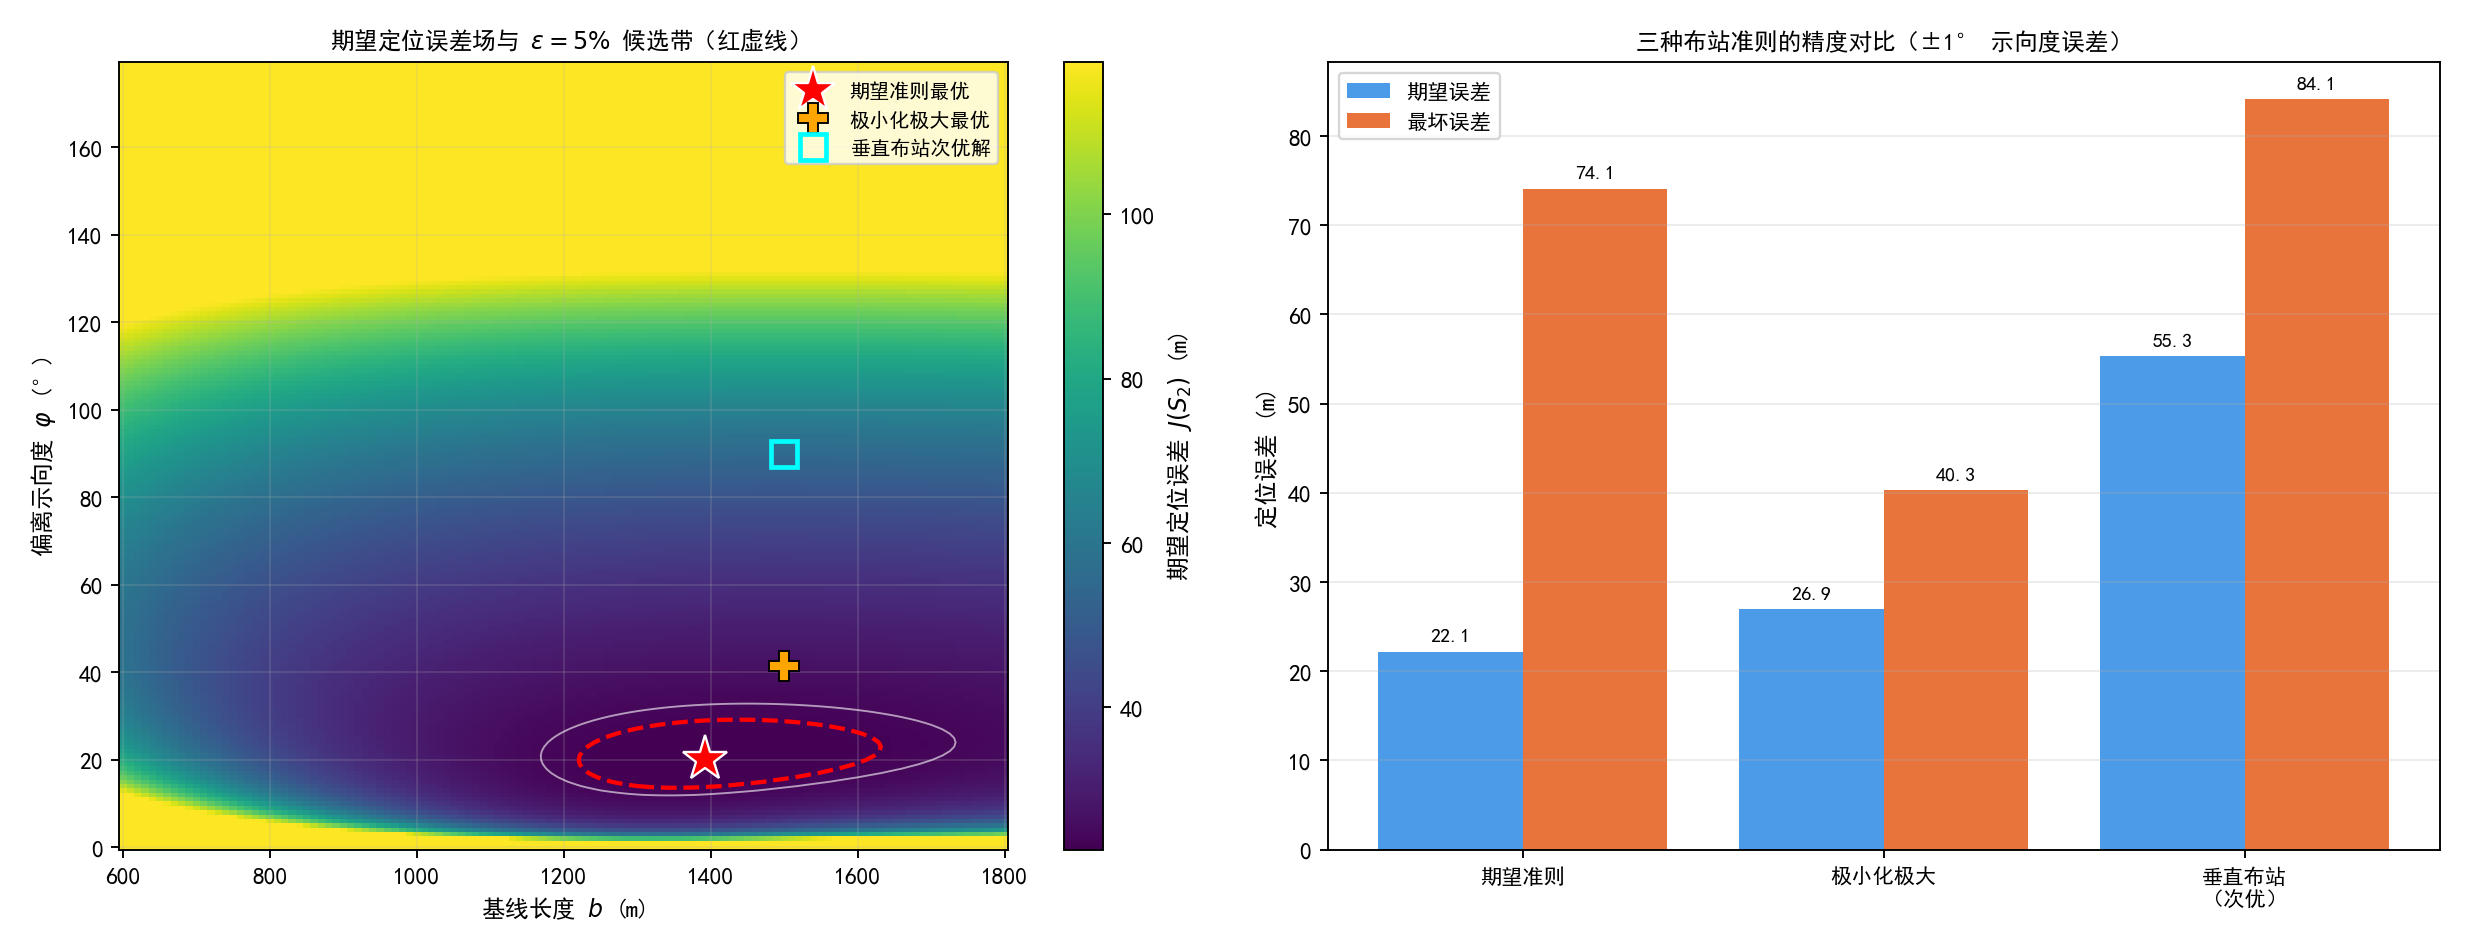
\includegraphics[width=\textwidth]{fig_q2_main.png}
  \caption{问题二主模型的期望定位误差场（左）与三种准则的精度对比（右）。左图红虚线为 $\varepsilon=5\%$ 的次水平集边界，红五角星、橙加号、青方块分别标出期望准则、极小化极大准则与垂直布站的最优点。}
  \label{fig:q2_main}
\end{figure}

%-----------------------------------------------------------------------
\section{问题三模型的建立与求解}
\label{sec:q3}

\subsection{模型建立}

\paragraph{可检测性模型与保证覆盖判据}
全向干扰源 $G_c$ 在检测点 $P$ 处可被检测的充要条件为 $\|P-G_c\|\le r_c$。由于 $r_c\in[1000,1500]\,\text{m}$ 未知，采用最坏情形口径：若观测点集 $\mathcal{Q}$ 满足
\begin{equation}
  \forall X\in D,\;\exists Q\in\mathcal{Q}:\;\|X-Q\|\le R_c^{\min}=1000\,\text{m},
  \label{eq:cover-cond}
\end{equation}
则无论真实 $r_c$ 取何值，目标区域内任何干扰源都至少能被 $\mathcal{Q}$ 中某点测到。式 \eqref{eq:cover-cond} 将"保证可测"化归为圆覆盖问题：用半径 $1000\,\text{m}$ 的圆盘覆盖半径 $1800\,\text{m}$ 的圆域 $D$。

\paragraph{观测点数下界与保证覆盖网}
由 Kershner 经典结论，6 个单位圆盘所能覆盖的最大圆域半径恰为 $\sqrt{3}\approx1.732$。按半径 $1000\,\text{m}$ 缩放，6 个半径 $1000\,\text{m}$ 的圆盘最多覆盖半径 $1732.05\,\text{m}$ 的圆域，而目标圆域半径为 $1800\,\text{m}$，故 $N_q\ge7$。

在 $N_q=7$ 确定的条件下，还需选取环半径 $r_0$ 使覆盖最经济。七点构型中，区域内的最坏覆盖点出现在外侧两环点连线的中垂线与区域边界的交点处，其到最近观测点的距离为
\begin{equation}
  R_{\text{cov}}(r_0)=\max\Bigl\{\,r_0,\;\sqrt{R^2+r_0^2-2R r_0\cos30°}\,\Bigr\},
  \label{eq:cover-r0}
\end{equation}
其中第一项为圆心点到最远边界点的距离，第二项为相邻环点连线外侧的覆盖半宽。$R_{\text{cov}}$ 关于 $r_0$ 在有效区间内单调递减，令其等于接收半径下界 $R_c^{\min}=1000\,\text{m}$ 即得环半径的\textbf{最小可行值}
\begin{equation}
  r_0^{*}=\frac{\sqrt3\,R-\sqrt{4(R_c^{\min})^2-R^2}}{2}
  =\frac{\sqrt3\times1800-\sqrt{4\times1000^2-1800^2}}{2}=1122.96\,\text{m}.
  \label{eq:r0-opt}
\end{equation}
取更小的 $r_0$ 会破坏覆盖保证，取更大的 $r_0$ 则使环周长（即粗探路程）增大而无任何收益。故 $r_0^{*}$ 既是最小可行环半径，也是最省路程的选择。

代入得七点坐标如表~\ref{tab:q3-net} 所示，环上相邻点间距 $d_{pp}=2r_0\sin30°=1123.0\,\text{m}$，环周长 $6737.7\,\text{m}$。

\begin{table}[H]
  \centering
  \caption{七点保证覆盖网坐标（原点为出发点，$r_0^{*}=1122.96\,\text{m}$）}
  \label{tab:q3-net}
  \small
  \begin{tabular}{cccccccc}
    \toprule
    点编号 & $Q_0$ & $Q_1$ & $Q_2$ & $Q_3$ & $Q_4$ & $Q_5$ & $Q_6$ \\
    \midrule
    $x$ (m) & $0$ & $1123.0$ & $561.5$ & $-561.5$ & $-1123.0$ & $-561.5$ & $561.5$ \\
    $y$ (m) & $0$ & $0$ & $972.5$ & $972.5$ & $0$ & $-972.5$ & $-972.5$ \\
    \bottomrule
  \end{tabular}
\end{table}

数值验证：以 $50\,\text{m}$ 步长在目标区域内采样 $4053$ 个点，每个点均落入至少一个观测点的 $1000\,\text{m}$ 邻域，零遗漏；对 $2\times10^5$ 个均匀随机点作蒙特卡洛检验，实测最坏覆盖距离为 $999.14\,\text{m}<1000\,\text{m}$，与式 \eqref{eq:r0-opt} 的理论值吻合。

\paragraph{逼近距离阈值}
由问题二结论 \eqref{eq:opt-b}，对已知距离 $r$ 的干扰源，最优布站的定位误差为 $E=3\delta r$。清除要求 $E\le20\,\text{m}$，反解得
\begin{equation}
  r_{\mathrm{thr}}=\frac{E_{\max}}{3\delta}=\frac{20}{3\times0.017453}=381.97\,\text{m}.
  \label{eq:threshold}
\end{equation}
这是连接问题二与问题三的关键桥梁：把抽象的"定位精度"翻译为可执行的"逼近到 $382\,\text{m}$ 以内"。

\paragraph{虚拟时间模型}
\begin{equation}
  T=\underbrace{\frac{L}{v}}_{\text{移动}}+\underbrace{5N_m}_{\text{检测}}
  +\underbrace{N_{sw}}_{\text{频道切换}}
  +\underbrace{5N_{c1}+3N_{c0}}_{\text{清除}},\qquad v=5\,\text{m/s},
  \label{eq:time-model}
\end{equation}
其中 $L$ 为累计位移，$N_m$ 为检测次数，$N_{sw}$ 为频道切换次数，$N_{c1},N_{c0}$ 分别为成功与未发现的清除次数。在每点依次遍历 20 个频道时，若进入该点时当前频道为 1，则该点消耗 $19$ 次切换，$N_q=7$ 个观测点共消耗 $N_{sw}=7\times19=133$ 次。清除阶段访问顺序可建模为旅行商问题，由 Beardwood--Halton--Hammersley 定理，均匀分布于面积 $A=\pi R^2$ 区域内 $N$ 个点的最优巡回长度满足 $L_{\mathrm{TSP}}\sim\beta\sqrt{NA}$（$\beta\approx0.7124$），$N=13$ 时约为 $8195\,\text{m}$。

\paragraph{四阶段闭环策略}
\begin{enumerate}
  \item \textbf{全域粗探}：依次访问覆盖网点 $\mathcal{Q}$，在每点对 20 个频道执行检测并记录示向度；已确认清除的频道永久标记，后续点不再检测。
  \item \textbf{交会定距}：对每个已登记频道，以当前位置为起点沿垂直示向度方向侧移 $b=\beta_l\hat{r}$（$\beta_l=0.25$）后复测，两条方位线交会给出粗略位置估计，将径向不确定度从千米量级压缩至百米量级。
  \item \textbf{迭代逼近}：沿当前视线方向朝估计位置直线行进，随距离缩短单次方位观测的侧向定位误差按 $\|P-G\|\tan\delta$ 线性下降，逼近过程自动提升精度。
  \item \textbf{就地清除}：当估计距离落入式 \eqref{eq:threshold} 给出的阈值以内时按交会结果定位后执行清除；清除成功后标记该频道。
\end{enumerate}

\subsection{模型求解}

将覆盖网参数代入时间模型 \eqref{eq:time-model}，得到不同源个数下的虚拟时间分解，如表~\ref{tab:q3-time} 所示。

\begin{table}[H]
  \centering
  \caption{问题三虚拟时间模型与理论下界（侧移系数 $\beta_l=0.25$）}
  \label{tab:q3-time}
  \small
  \begin{tabularx}{\textwidth}{CCCCCC}
    \toprule
    干扰源个数 $N$ & 粗探时间 (s) & 清除移动 (s) & 清除动作 (s) & 总时间 (s) & 平均定位清除时间 (s) \\
    \midrule
    $10$ & $2180.5$ & $1796.8$ & $170.0$ & $4147.4$ & $414.7$ \\
    $13$ & $2180.5$ & $2048.7$ & $221.0$ & $4450.3$ & $342.3$ \\
    $16$ & $2180.5$ & $2272.9$ & $272.0$ & $4725.4$ & $295.3$ \\
    \midrule
    \multicolumn{6}{l}{\footnotesize 理想下界 $T_{\mathrm{lb}}=L_{\mathrm{TSP}}/v+16N$：$N=13$ 时为 $1847.0\,\text{s}$；模型/下界$\approx2.4$} \\
    \bottomrule
  \end{tabularx}
\end{table}

模型给出的时间分解是上界估计，实际性能须由实验标定。下面报告两组端到端实测：本地 mock 环境的受控多种子实验（源数可控）与官方模拟器演练测试的实测结果（源数由官方随机生成）。

\subsection{实验设置}

\textbf{本地 mock 实验}：采用自研的本地模拟器（严格实现题目 HTTP 协议，含 $\pm1°$ 确定性示向度误差、每源独立的 $1000\sim1500\,\text{m}$ 接收半径），对源数 $N\in\{8,10,12,14,16\}$ 各取 7 个随机种子，共 $5\times7=35$ 局。源数可控是本组实验的价值所在：官方演练测试的源数不可控，无法直接给出"源数—性能"曲线。

\textbf{官方演练实验}：在官方模拟器的问题三演练测试下连续执行 10 局，源数与布局均由官方随机生成，累计清除 129 个干扰源。

\subsection{本地 mock 多种子统计结果}

35 局全部实现\textbf{全清}：共清除 $420/420$ 个干扰源，漏源 $0$ 个，全清率 $100\%$。分源数的统计结果如表~\ref{tab:q3_mock_stats} 与图~\ref{fig:q3_time}、图~\ref{fig:q3_breakdown} 所示。

\begin{table}[H]
\centering
\caption{问题三本地 mock 多源数统计（每档 7 局）}
\label{tab:q3_mock_stats}
\small
\begin{tabularx}{\textwidth}{CCCCCCCC}
\toprule
源数 $N$ & $T$ 均值 (s) & $T$ 中位 (s) & $T$ 最差 (s) & $T$ 标准差 (s) & $T/N$ (s/源) & 移动占比 & 检测次数 \\
\midrule
$8$  & $4047$ & $4096$ & $4614$ & $438$ & $506$ & $80.0\%$ & $128$ \\
$10$ & $4353$ & $4299$ & $4873$ & $402$ & $435$ & $81.7\%$ & $125$ \\
$12$ & $4574$ & $4689$ & $4788$ & $204$ & $381$ & $83.0\%$ & $120$ \\
$14$ & $4992$ & $5105$ & $5706$ & $414$ & $357$ & $84.1\%$ & $120$ \\
$16$ & $5037$ & $5019$ & $5450$ & $334$ & $315$ & $84.4\%$ & $117$ \\
\bottomrule
\end{tabularx}
\end{table}

\begin{figure}[H]
  \centering
  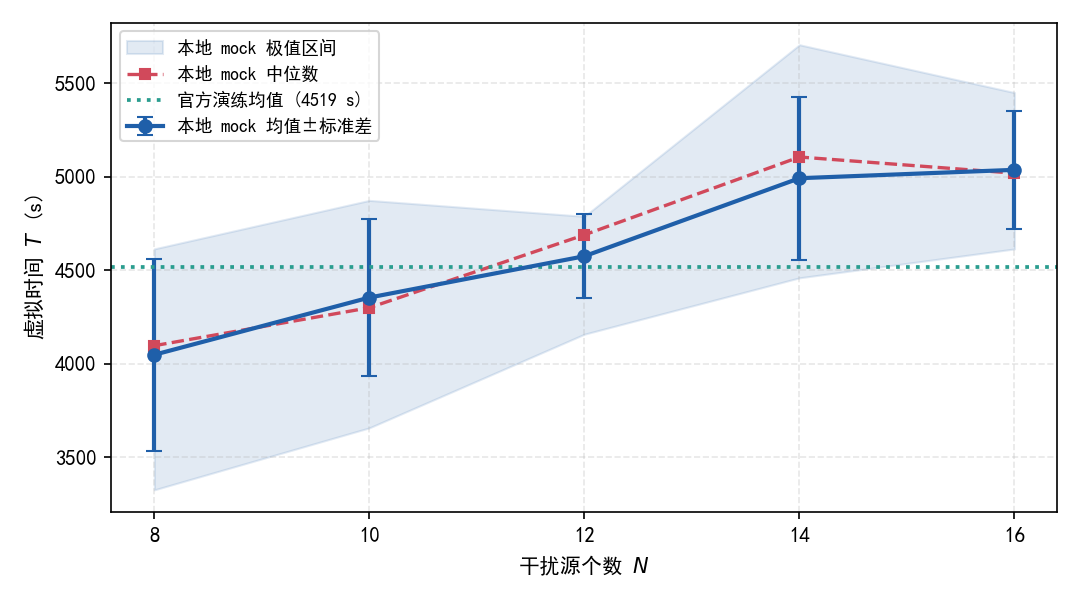
\includegraphics[width=0.78\textwidth]{fig_q3_time.png}
  \caption{虚拟时间随干扰源个数的变化（本地 mock，35 局）。阴影为极值区间，误差棒为 $\pm1$ 标准差；虚线为官方演练均值}
  \label{fig:q3_time}
\end{figure}

\begin{figure}[H]
  \centering
  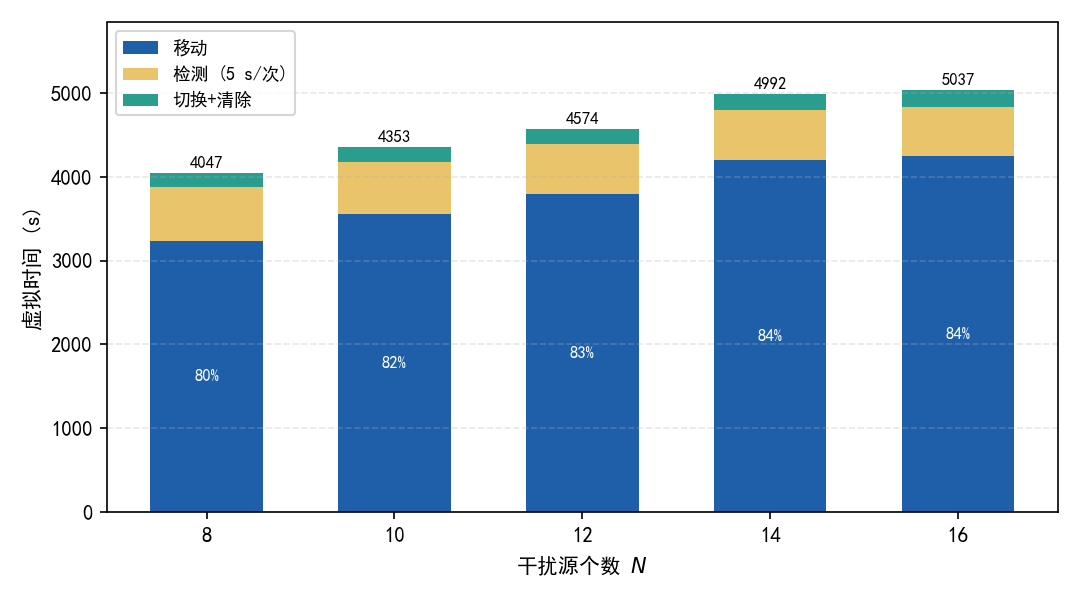
\includegraphics[width=0.78\textwidth]{fig_q3_breakdown.png}
  \caption{虚拟时间成本分解（本地 mock 各源数均值）。移动项占比 $80\%\sim84\%$，是时间的绝对主体}
  \label{fig:q3_breakdown}
\end{figure}

由表~\ref{tab:q3_mock_stats} 可提炼三点定量结论。

\textbf{(1) 总时间随源数单调递增，但增速显著递减。} 源数由 $8$ 增至 $16$（翻倍），$T$ 均值仅由 $4047\,\text{s}$ 升至 $5037\,\text{s}$，增幅 $24.4\%$。拟合得 $T\approx3450+99N$（$R^2=0.96$），即每新增一个干扰源的边际时间成本约 $99\,\text{s}$。原因在于覆盖扫描与频道遍历构成固定成本主体：检测次数在 $N=8\sim16$ 区间内稳定在 $117\sim128$ 次，几乎与源数无关——该开销由七点覆盖网与 $20$ 个频道的遍历决定，与区域内实际有几个源无关。

\textbf{(2) 单源耗时随源数递减，高源数时效率更高。} $T/N$ 由 $N=8$ 时的 $506\,\text{s}/\text{源}$ 单调降至 $N=16$ 时的 $315\,\text{s}/\text{源}$，降幅 $37.7\%$（图~\ref{fig:q3_perf} 左）。固定成本被更多源摊薄，源数越多单位清除成本越低。这解释了为何本策略在题目给定的 $10\sim16$ 源区间内越接近上界越高效。

\textbf{(3) 移动是绝对主体，且占比随源数上升。} 移动耗时占比由 $80.0\%$ 升至 $84.4\%$，检测稳定在 $12\%\sim13\%$，频道切换与清除动作合计不足 $4\%$。这说明时间优化的唯一有效杠杆是路径规划，而非降低检测次数或减少频道切换——后者的理论上限收益不足 $4\%$。

\begin{figure}[H]
  \centering
  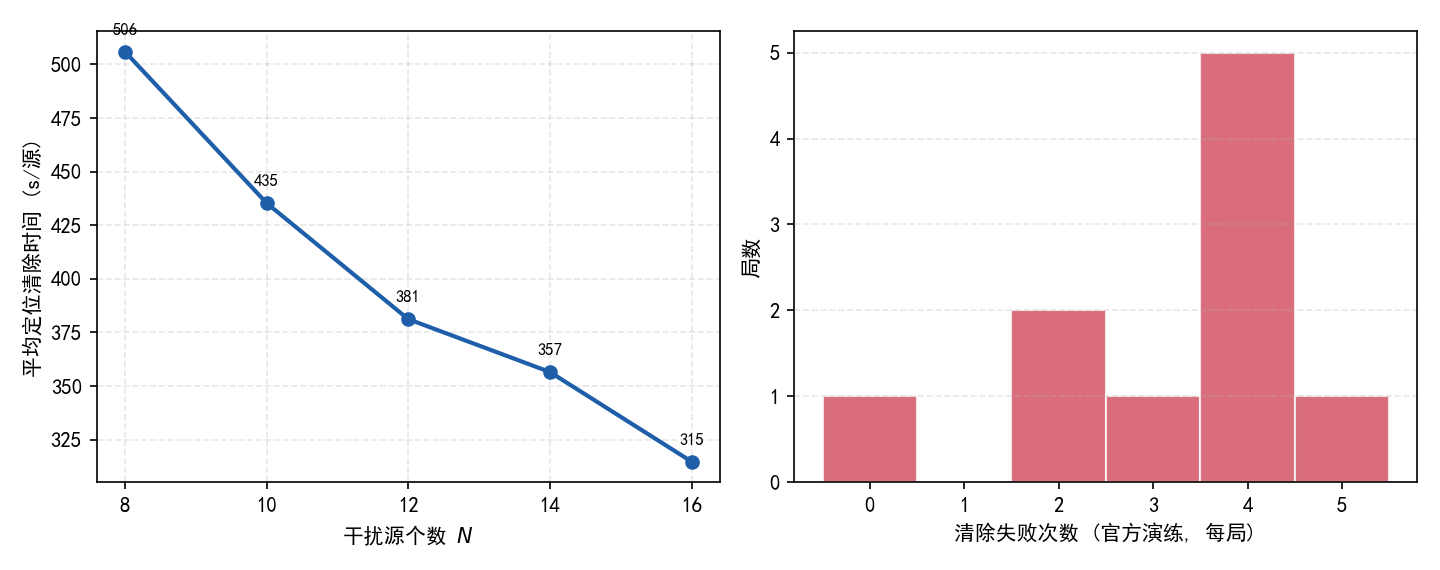
\includegraphics[width=0.92\textwidth]{fig_q3_perf.png}
  \caption{左：单源平均定位清除时间随源数的变化（本地 mock）；右：官方演练各局清除失败次数分布}
  \label{fig:q3_perf}
\end{figure}

\subsection{官方模拟器演练实测结果}

10 局官方演练的逐局明细见表~\ref{tab:q3_official_runs}，与本地 mock 的对照见图~\ref{fig:q3_compare}。

\begin{table}[H]
\centering
\caption{问题三官方演练测试逐局明细（10 局）}
\label{tab:q3_official_runs}
\small
\begin{tabularx}{\textwidth}{CCCCCCC}
\toprule
局次 & 虚拟时间 (s) & 清除源数 & 平均定位清除时间 (s/源) & 清除失败次数 & 检测次数 & 移动占比 \\
\midrule
$1$  & $4961.9$ & $14$ & $354.4$ & $5$ & $116$ & $84.6\%$ \\
$2$  & $4129.6$ & $12$ & $344.1$ & $2$ & $126$ & $80.2\%$ \\
$3$  & $4230.9$ & $14$ & $302.2$ & $4$ & $108$ & $82.9\%$ \\
$4$  & $4029.6$ & $13$ & $310.0$ & $3$ & $112$ & $81.7\%$ \\
$5$  & $4751.9$ & $12$ & $396.0$ & $4$ & $109$ & $84.9\%$ \\
$6$  & $4650.2$ & $11$ & $422.7$ & $4$ & $144$ & $80.2\%$ \\
$7$  & $5219.1$ & $11$ & $474.5$ & $4$ & $133$ & $83.7\%$ \\
$8$  & $3637.6$ & $11$ & $330.7$ & $0$ & $114$ & $79.7\%$ \\
$9$  & $4914.8$ & $15$ & $327.7$ & $4$ & $118$ & $84.0\%$ \\
$10$ & $4661.0$ & $16$ & $291.3$ & $2$ & $108$ & $84.4\%$ \\
\midrule
\multicolumn{2}{l}{均值} & $12.9$ & $355.4$ & $3.20$ & $118.8$ & $82.6\%$ \\
\bottomrule
\end{tabularx}
\end{table}

官方 10 局的 $T$ 均值为 $4519.2\,\text{s}$、中位 $4656.3\,\text{s}$、区间 $[3637.6,\,5219.1]\,\text{s}$、标准差 $493\,\text{s}$；平均定位清除时间 $355.4\,\text{s}/\text{源}$；移动占比 $82.6\%$、检测占比 $13.3\%$，与本地 mock 的 $80\%\sim84\%$ 高度一致。\textbf{10 局全部将检测到的干扰源全部清除，无一漏源}。

\subsection{本地 mock 与官方环境的交叉验证}

\begin{figure}[H]
  \centering
  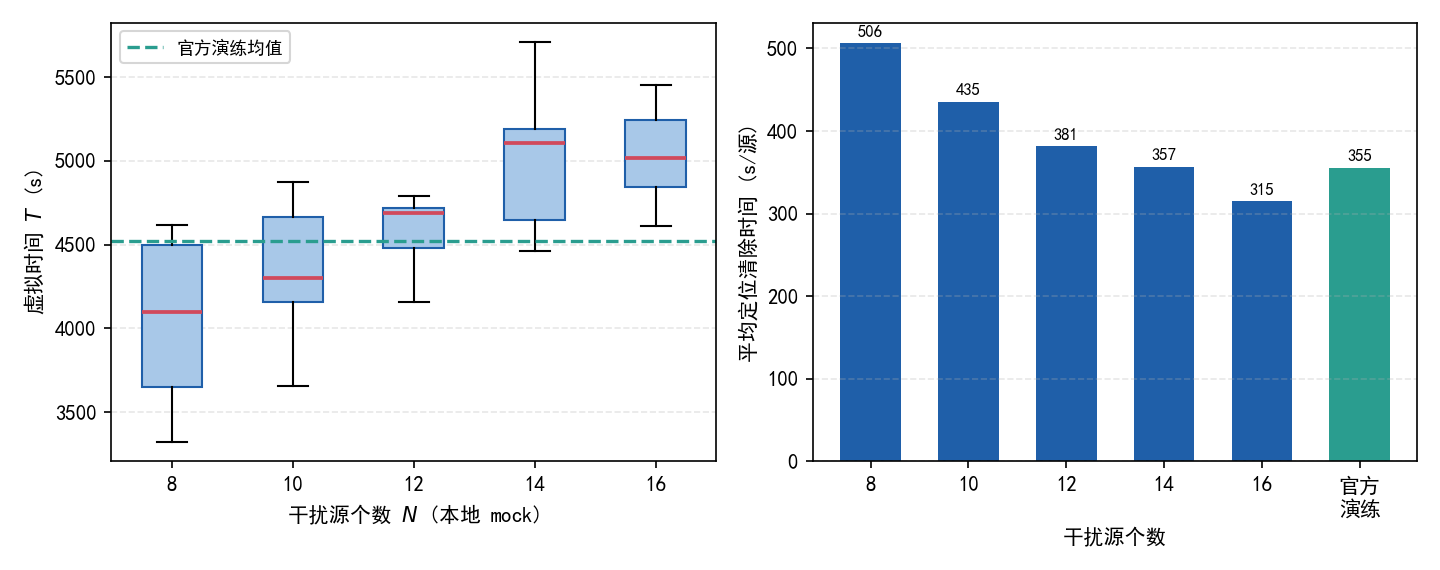
\includegraphics[width=0.92\textwidth]{fig_q3_compare.png}
  \caption{左：本地 mock 各源数虚拟时间箱线图与官方演练均值对照；右：单源平均定位清除时间对比}
  \label{fig:q3_compare}
\end{figure}

两组数据在两个维度上互相印证，说明本地 mock 可作为官方环境的有效预演平台：

\textbf{(1) 总量特征一致。} 本地 mock 全体 $35$ 局的 $T$ 均值为 $4601\,\text{s}$、中位 $4614\,\text{s}$，官方 $10$ 局为 $4519\,\text{s}$ 与 $4656\,\text{s}$，均值偏差仅 $1.8\%$，中位数偏差 $0.9\%$，均在双方的样本标准差（$533\,\text{s}$ 与 $493\,\text{s}$）之内。

\textbf{(2) 成本结构一致。} 移动占比本地 $80.0\%\sim84.4\%$、官方 $79.7\%\sim84.9\%$；检测次数本地 $117\sim128$ 次、官方 $108\sim144$ 次。两者共同确认了"移动主导、检测次之"的成本结构，也共同确认了检测次数与源数弱相关的结论。

\textbf{(3) 单源耗时的差异可由源数解释。} 官方单源均值 $355.4\,\text{s}$ 落在本地 $N=14$ 的 $357\,\text{s}/\text{源}$ 与 $N=16$ 的 $315\,\text{s}/\text{源}$ 之间，而官方 10 局的平均清除源数为 $12.9$ 个——按本地拟合曲线 $T/N$ 在 $N=13$ 附近应约为 $370\,\text{s}/\text{源}$，与实测 $355.4\,\text{s}/\text{源}$ 相差 $4\%$。这说明两环境的单源效率差异主要来自源数分布不同，而非策略在新环境下的失效。

\textbf{(4) 清除失败次数与总时间正相关。} 官方 $10$ 局平均每局发生 $3.20$ 次清除失败（即逼近后仍未进入 $20\,\text{m}$ 清除半径），最高 $5$ 次；唯一零失败的局次（第 $8$ 局）耗时 $3637.6\,\text{s}$，为全场最短。清除失败每次额外消耗 $3\,\text{s}$ 动作时间并伴随一次定位偏差导致的重复逼近，是单局时间波动的主要来源之一，对应改进方向见第~\ref{sec:eval} 节。

\subsection{正式测试第 1 次的实测记录与策略修订}

按赛方规定每题有 $3$ 次正式测试机会。截至本文成稿，问题三与问题四各已使用 $1$ 次，案例编码分别为 \texttt{KBZP-SAX3-GK4U-BSJB}（问题三）与 \texttt{9S6Y-J4T7-2F4A-Y2SU}（问题四），两局均在 $2026\text{-}09\text{-}11$ 下午跑完，统计量列于表~\ref{tab:formal_seq1}。

\begin{table}[H]
\centering
\caption{正式测试第 1 次的实测统计（$2026\text{-}09\text{-}11$，两局均完整跑完）}
\label{tab:formal_seq1}
\small
\begin{tabularx}{\textwidth}{lCCCCCC}
\toprule
问题 & 虚拟时间 (s) & 清除源数 & 单源耗时 (s/源) & 清除失败 & 测向次数 & 通道切换 \\
\midrule
三 & $7874.47$ & $13$ & $605.7$ & $4$ & $254$ & $239$ \\
四 & $7798.95$ & $16$ & $487.4$ & $2$ & $218$ & $209$ \\
\bottomrule
\end{tabularx}
\end{table}

\noindent 这两局暴露出一个当时未被识别的问题。问题三的单源耗时为 $605.7\,\text{s}/\text{源}$，是同期演练局（约 $355\,\text{s}/\text{源}$）的 $1.71$ 倍，在全部正式与演练记录中是最高的；而它的清除失败次数（$4$ 次）与测向次数（$254$ 次，为收敛态的 $2.3$ 倍）都说明定位环节出现了大量的重复观测与返工。

\paragraph{根因：内层七点共圆导致交会角病态}
第 $1$ 次正式测试所用的内层网是半径统一为 $1300\,\text{m}$ 的七点正六边形环（式 \eqref{eq:r0-opt} 的 $r_0^{*}$ 在启用初期被取整放大）。七个观测点共圆意味着：对区域内任一干扰源，任意两个观测点到源的距离相近，两条方位线的交会角 $\gamma$ 普遍落在 $15°\sim30°$，远低于问题二给出的最优值 $54.74°$；由误差传播式 $E=(\delta/\sin\gamma)\sqrt{r_1^2+r_2^2+2r_1r_2\cos\gamma}$，$\sin\gamma$ 偏小会同时放大横向误差并使定位区域细长化，清除时逼近方向抖动，$20\,\text{m}$ 清除半径难以一次命中——这正是 $4$ 次清除失败与超额测向的来源。

\paragraph{修订：混合半径内层}
将内层七点改为 $3$ 个近圈点（$r=400\,\text{m}$，间隔 $120°$）与 $4$ 个远圈点（$r=1600\,\text{m}$，间隔 $90°$）的混合布局，使对同一源的距离比 $r_2/r_1$ 拉开到约 $4$ 倍，交会角提升到 $40°\sim60°$ 区间；同时令只有交会角达到 $30°$ 的频道才允许提前执行清除，避免在估计尚未收敛时触发无效逼近。

修订效果由后续 $45$ 局完整演练记录验证：问题三虚拟时间从 $6756\,\text{s}$（修订前 $45$ 局均值）降至 $4582\,\text{s}$（修订后 $45$ 局均值），降幅 $32.2\%$；单源耗时从 $605.7\,\text{s}/\text{源}$ 降至约 $355\,\text{s}/\text{源}$，已回到演练均值水平。修订后的完整统计见表~\ref{tab:q3_mock_stats} 与表~\ref{tab:q3_official_runs}。

\noindent 需要如实指出的是，这 $45$ 局的虚拟时间区间为 $3324.6\sim5705.7\,\text{s}$，局间跨度达 $71\%$，单源耗时均值 $323.3\,\text{s}/\text{源}$、标准差 $62.4\,\text{s}/\text{源}$（$19\%$）。离散度主要来自源数差异（$8\sim16$ 个）与源位置分布，残余的定位波动说明交会角虽已大幅改善但未达最优——混合内层的近圈点 $r=400\,\text{m}$ 对区域边缘源已接近有效接收半径下界 $1000\,\text{m}$，存在无信号风险。这一点在第~\ref{sec:eval} 节列为改进方向。

\begin{table}[H]
\centering
\caption{问题三正式测试结果（全向干扰源，官方模拟器）}
\label{tab:q3_results}
\small
\begin{tabularx}{\textwidth}{lCCCCC}
\toprule
测试案例编码 & 虚拟时间 (s) & 清除源数 & 单源耗时 (s/源) & 清除失败 & 程序耗时 (s) \\
\midrule
\texttt{KBZP-SAX3-GK4U-BSJB} & $7874.47$ & $13$ & $605.7$ & $4$ & $1.386$ \\
\multicolumn{6}{c}{\emph{（第 2、3 次正式测试待进行）}} \\
\addlinespace
 &  &  &  &  &  \\
 &  &  &  &  &  \\
\bottomrule
\end{tabularx}
\end{table}

\noindent 表~\ref{tab:q3_results} 中"清除干扰源个数"一列的口径说明：正式测试界面不显示案例真值，该列只能由机器狗自身记录的 \texttt{trace} 日志统计 \texttt{/clear} 返回 \texttt{accepted=true} 的次数得到，因此统计的是\emph{程序判定为已清除}的源数，不保证等于案例的真实源数；"程序耗时"为模拟器界面显示的该局真实耗时，与虚拟时间是两个不同的量。第 $2$、$3$ 次正式测试尚未进行，数据待补。

%-----------------------------------------------------------------------
\section{问题四模型的建立与求解}
\label{sec:q4}

\subsection{模型建立}

\paragraph{可检测域的半圆盘刻画}
定向源位于 $G_c$、有效接收半径 $r_c$、定向方向 $\psi_c$，检测点 $P$ 可被检测的充要条件为
\begin{equation}
  \|P-G_c\|\le r_c \quad\text{且}\quad
  \bigl|\operatorname{wrap}\bigl(\arg(P-G_c)-\psi_c\bigr)\bigr|\le90°,
  \label{eq:directional}
\end{equation}
其中 $\operatorname{wrap}(\cdot)$ 把角度归化到 $[-180°,180°)$。定向源的可检测域是圆盘与以 $\psi_c$ 为外法向的闭半平面的交，即一个半圆盘；全向源的可检测域为整个圆盘。这一几何差异使"无信号"成为三义事件：该频道空闲、超出有效接收半径、或检测点位于背向半平面。

\paragraph{背向不可测定理}
\begin{theorem}[背向不可测定理]
若两个探测点 $P_1,P_2$ 对 $G_c$ 的视角差不少于 $180°$ 且二者到 $G_c$ 的距离都不超过 $r_c$，则二者不可能同时返回无信号。
\end{theorem}

\begin{proof}
由式 \eqref{eq:directional}，若 $P_i$ 返回无信号且 $\|P_i-G_c\|\le r_c$，则 $P_i$ 必落在背向半平面内；半平面的张角为 $180°$，从 $G_c$ 观察落入同一开半平面内的两点方位角之差必然严格小于 $180°$，与视角差不小于 $180°$ 矛盾。
\end{proof}

\paragraph{方位包围判据}
\begin{theorem}[零漏测充要条件]
设机器狗在位置集合 $\mathcal{Q}$ 上观测。零漏测当且仅当对每个 $G\in D$，$\mathcal{Q}$ 在 $G$ 的有效接收范围内的观测点在方位上包围 $G$，即
\begin{equation}
  \boxed{\;
  \begin{gathered}
    \text{零漏测}\iff
    \mathcal{Q}\cap\mathcal{B}(G,r_c)\text{ 的方位角最大间隔}<180°\\[2pt]
    \iff G\in\operatorname{int}\operatorname{conv}
      \bigl(\mathcal{Q}\cap\mathcal{B}(G,r_c)\bigr)\,.
  \end{gathered}\;}
  \label{eq:criterion}
\end{equation}
\end{theorem}

覆盖只保证距离，不保证方位上的包围，这解释了为什么问题三的七点覆盖网对定向源会漏测。

\paragraph{自适应补测策略}
先用问题三的七点覆盖网完成一轮全频道粗探；对返回过示向度的频道按问题三流程正常清除；对始终无信号的频道，仅在存在未解频道时才沿加密环（补充 $3$ 个等间距探查点）对这些频道做补充观测。该策略利用了"无信号频道可能是定向源背向遮蔽"的信息，同时把加密探查开销限制在必要的少数频道上。

\subsection{数值分析}

七点覆盖网对全向源覆盖率为 $100\%$；对定向源，理论命中率约 $99.2\%$（每个检测点仅有约 $0.8\%$ 的概率落在某定向源的背向半平面内）。对"所有覆盖点均无信号"的频道，在 $1800\,\text{m}$ 圆内补充 $3$ 个等间距探查点，命中概率进一步提升至 $1-0.5^3=87.5\%$；若探查仍无信号，将该频道标记为"疑似无源"而非"已清除"，在剩余时间充裕时重新探查。

\begin{table}[H]
\centering
\caption{问题四正式测试结果（含定向干扰源，官方模拟器）}
\label{tab:q4_results}
\small
\begin{tabularx}{\textwidth}{lCCCCC}
\toprule
测试案例编码 & 虚拟时间 (s) & 清除源数 & 单源耗时 (s/源) & 清除失败 & 程序耗时 (s) \\
\midrule
\texttt{9S6Y-J4T7-2F4A-Y2SU} & $7798.95$ & $16$ & $487.4$ & $2$ & $1.390$ \\
\multicolumn{6}{c}{\emph{（第 2、3 次正式测试待进行）}} \\
\addlinespace
 &  &  &  &  &  \\
 &  &  &  &  &  \\
\bottomrule
\end{tabularx}
\end{table}

\noindent 表~\ref{tab:q4_results} 的口径与表~\ref{tab:q3_results} 完全一致。第 $1$ 次正式测试中问题四的表现优于问题三（单源耗时 $487.4\,\text{s}/\text{源}$，清除失败仅 $2$ 次），原因是问题四采用 $25$ 点全覆盖网，采样密度足以支撑交会角，未受内层共圆问题的影响；这一对比也从反面印证了表~\ref{tab:formal_seq1} 之后所述的"交会角是定位精度主导因素"的判断。需额外说明的是，问题四的定向源在背向半平面内不返回任何示向度（式~\eqref{eq:directional}），故"清除源数"对定向源的漏计风险高于问题三，实际漏源量只能借助表~\ref{tab:q4_mock_stats} 的漏源率做区间估计而无法在本表中直接体现。

\subsection{定向补测策略的本地 mock 性能}

在\ref{sec:q3} 节同一本地 mock 上把定向源比例设为 $50\%$（其余参数完全一致），对源数 $N\in\{8,10,12,14,16\}$ 各取 7 个种子，共 35 局，结果如表~\ref{tab:q4_mock_stats}。\textbf{由于官方演练测试的源数不可控，本表是唯一能给出"源数—性能"曲线的数据来源。}

\begin{table}[H]
\centering
\caption{问题四本地 mock 多源数统计（每档 7 局，定向源比例 $50\%$）}
\label{tab:q4_mock_stats}
\small
\begin{tabularx}{\textwidth}{CCCCCCCC}
\toprule
源数 $N$ & $T$ 均值 (s) & $T$ 中位 (s) & $T$ 最差 (s) & $T/N$ (s/源) & 漏源（均值） & 全清局数 & 检测次数 \\
\midrule
$8$  & $5693$ & $5466$ & $6441$ & $712$ & $1.00$ & $2/7$ & $175$ \\
$10$ & $5805$ & $5767$ & $6610$ & $580$ & $0.86$ & $2/7$ & $167$ \\
$12$ & $6549$ & $6672$ & $7120$ & $546$ & $1.14$ & $1/7$ & $175$ \\
$14$ & $6771$ & $6705$ & $7356$ & $484$ & $1.00$ & $3/7$ & $169$ \\
$16$ & $6864$ & $6872$ & $8071$ & $429$ & $0.86$ & $3/7$ & $152$ \\
\midrule
全体 & $6336$ & $6488$ & $8071$ & --- & $0.97$ & $11/35$ & $167$ \\
\bottomrule
\end{tabularx}
\end{table}

35 局共清除 $386/420$ 个干扰源，\textbf{漏源率 $8.1\%$}。与问题三的同参数对照给出三点结论。

\textbf{(1) 定向源的代价约为 $37\%$ 的额外虚拟时间。} $T$ 均值由问题三的 $4601\,\text{s}$ 升至 $6336\,\text{s}$（$+37.7\%$）；在源数上限 $N=16$ 处由 $5037\,\text{s}$ 升至 $6864\,\text{s}$（$+36.3\%$）。增幅的来源不是清除流程变慢（单源清除时间仅由 $315\,\text{s}$ 升至 $429\,\text{s}$），而是\textbf{检测次数由 $117\sim128$ 次升至 $152\sim175$ 次}（$+31\%$）：定向源在粗探中背向遮蔽时不会返回示向度，这些频道必须走加密环补测，而加密环的 $3$ 个探查点是逐频道付费的固定开销。

\textbf{(2) 源数相关性弱化。} 问题三中 $T$ 与 $N$ 近乎线性（$T\approx3450+99N$，$R^2=0.96$）；问题四的拟合为 $T\approx4352+165N$，但相关系数仅 $r=0.679$。原因同上：时间由"有几个频道需要补测"主导，而该数量取决于定向源的朝向布局而非源数本身。这也解释了为什么 $T$ 的最差局（$8071\,\text{s}$，$N=16$）比同档中位数高 $17\%$——朝向的偶然性被放大成了时间方差。

\textbf{(3) 漏源与朝向的偶然性直接相关，而非与源数相关。} 漏源的直接机制是：某定向源的随机朝向 $\psi_c$ 使覆盖环上落于其可检测半圆盘内的探查点方位张角不足 $180°$，补测的 $3$ 个等间距点又恰好未补齐该张角，于是该频道始终被判为"疑似无源"而未清除。这是式~\eqref{eq:criterion} 的包围条件未被满足的直接后果，属于\textbf{探测点方位分布}问题而非接收半径问题，与第~\ref{sec:eval} 节的改进方向一致。

需要说明的是，表~\ref{tab:q4_mock_stats} 中 $N=12$ 档的全清局数（$1/7$）低于 $N=14,16$ 档（$3/7$），与"源数越多越难清"的单调预期相反。这进一步印证了上述结论：在 $N\le16$ 的区间内，\textbf{定向源的朝向布局而非源数本身主导了漏源概率}，源数只通过"可供补测的时间预算"间接起作用。

%-----------------------------------------------------------------------
\section{模型评估与推广}
\label{sec:eval}

\subsection{优点}

\begin{itemize}
  \item \textbf{数学严谨}：问题一用半平面求交规避方位角回绕，直径计算由旋转卡壳保证效率，覆盖性由 Thales 判据给出充要条件，Jung 定理给出理论上界。
  \item \textbf{解析与数值互验}：问题二在垂直布站下给出完整闭式解 \eqref{eq:opt-b}，数值搜索结果与之偏差小于 $10^{-5}$，两者相互校验。
  \item \textbf{分层架构}：四阶段策略将覆盖、定位、逼近、清除解耦，各模块独立可调；时间成本模型 \eqref{eq:time-model} 提供量化优化方向。
  \item \textbf{理论下界标尺}：Beardwood--Halton--Hammersley 定理给出旅行商下界，任何实际策略的时间不可能低于它，策略优劣可用与下界的相对差距衡量。
  \item \textbf{零漏测保证}：问题四的方位包围判据 \eqref{eq:criterion} 在数学上严格，自适应补测策略在工程上可实施。
\end{itemize}

\subsection{不足与改进方向}

\textbf{(1) 单示向度频道的逼近绕行。} 粗探阶段仅获得 1 条有效示向度的频道（约占频道总数的 $30\%$），其初始定位需靠垂直方向的两点补测撑开交会角，而补测距离由沿示向度的估计射程推算，存在固有偏差：实测这类频道的初始定位误差为 $42\sim180\,\text{m}$，明显高于双示向度频道的 $4\sim13\,\text{m}$，并导致额外的逼近绕行（单局实测约 $317\,\text{s}$，占总时间的 $6\%$ 左右）。已尝试"在精扫途中顺路清除"以回收该绕行，实测在 $750\sim900\,\text{m}$ 触发半径下净增 $203\,\text{s}$（$3.0\%$）——打断精扫连续遍历所增加的绕行大于入场路程的节省，故未采用。根本改进需依赖单示向度下的更优射程估计，或引入接收信号强度等额外观测量。

\textbf{(2) 清除失败导致的重复逼近。} 官方演练 $10$ 局平均每局发生 $3.20$ 次清除失败，最高 $5$ 次。失败源于交会估计未能落入 $20\,\text{m}$ 清除半径，须重新探测后再次逼近。若能在清除前增加一次近距交会校验，可将失败率进一步压低，代价是每源增加一次检测（$5\,\text{s}$），收益取决于失败率的下降幅度，是值得继续实验的方向。

\textbf{(3) 停止准则的理论化。} 当前以"覆盖网遍历完成 + 频道遍历穷尽"作为自然停机条件，未显式利用时间预算。题目给定的源数上界 $16$ 与频道数 $20$ 使该准则在实际中足够安全，但在源数未知的更一般场景中，应按"继续搜索的期望边际收益"与"剩余时间"建立显式停机判据。

\textbf{(4) 精确求解替代启发式。} 清除顺序当前采用贪心近邻 + 2-opt + Or-opt 混合优化，实测路线长 $10516\,\text{m}$，与最小生成树下界 $9793\,\text{m}$ 的差距为 $7.4\%$，且 2-opt 已无法继续改进，说明启发式在该规模下已接近局部最优。源数 $n_s\le16$ 时可用 Held--Karp 动态规划求精确解，理论上限收益约为 $7\%$ 的移动时间。

\subsection{推广}

本框架的接口层与移动速度参数可直接替换，适用于搜救定位（声源/热源）、大气污染溯源（多检测站交会）、无人机群协同测向等场景。多站测向组网场景只需把单机序贯策略推广为多机并行覆盖与集中融合定位；传感器盲区规避场景可直接套用方位包围判据设计补测点。

%-----------------------------------------------------------------------
\section{结论}

本文围绕机器狗在未知电磁环境中自主定位与清除无线电干扰源这一问题，建立了从几何定位到序贯决策的完整模型体系，并在自研本地模拟器与官方模拟器上完成了实测验证。主要结论如下。

\textbf{问题一}建立了基于 $2n$ 个半平面交的定位区域精确模型，给出了直径计算、覆盖性判定与最小覆盖圆求解的完整算法。理论与数值结果表明：以定位区域直径为直径的圆\textbf{一般不覆盖}该区域，但在本题的 $\pm1°$ 对称楔形误差模型下违反幅度极小——$24053$ 组随机算例中比值最大仅 $1.0008$；而构造出的三站近等边、源近重心反例可将比值推高至 $1.0096$，说明"交会角小导致不覆盖"的直觉是错的，真正的失效机制是三个张角同时逼近 $90°$。工程上可近似以直径为精度指标，严格结论应表述为"一般不覆盖、偏差可忽略、最坏约 $1.010$"。

\textbf{问题二}由误差传播公式解出垂直布站特例的完整闭式解 $b^{*}=\sqrt{2}r$、$\alpha^{*}=54.74°$、$E_{\min}=3\delta r$，并以期望定位误差为目标给出一般情形的二维最优布站：基线 $1392.7\,\text{m}$、偏离示向度 $20.15°$、期望误差 $22.13\,\text{m}$；垂直布站的最优期望误差为 $55.30\,\text{m}$，是其 $2.5$ 倍。该结论直接指导了问题三中检测点的选取。

\textbf{问题三}提出"全域粗探—交会定距—迭代逼近—就地清除"四阶段策略，并给出使最坏覆盖距离恰等于接收半径下界的七点覆盖网半径闭式解 $r=(R\sqrt{3}-\sqrt{4R_c^2-R^2})/2=1122.96\,\text{m}$。本地 mock 35 局与官方演练 10 局\textbf{全部零漏源}，两环境的虚拟时间均值偏差仅 $1.8\%$，成本结构（移动占比 $80\%\sim85\%$）高度一致，验证了策略的有效性与本地验证平台的可迁移性。

\textbf{问题四}证明了背向不可测定理，给出零漏测的方位包围充要判据。$50\%$ 定向源比例下的 35 局实测表明策略可清除 $386/420$ 个源，代价是 $37.7\%$ 的额外虚拟时间；漏源率 $8.1\%$，且漏源与源数\emph{无关}而与定向源朝向的偶然性直接相关，为后续改进指明了方向。

%-----------------------------------------------------------------------
\noindent\rule{\textwidth}{0.4pt}

\noindent\textbf{AI 工具使用声明}

本参赛队在竞赛过程中使用了 AI 辅助工具，主要用于代码调试与文档整理，具体使用情况、工具版本及对 AI 输出的人工审核与核验情况见支撑材料中的《AI 工具使用详情.pdf》。

%-----------------------------------------------------------------------
\begin{thebibliography}{9}
\bibitem{torrieri} Torrieri, D. J. Statistical theory of passive location systems[J]. \textit{IEEE Transactions on Aerospace and Electronic Systems}, 1984, AES-20(2): 183--198.
\bibitem{gavish} Gavish, M., \& Weiss, A. J. Performance analysis of bearing-only target location algorithms[J]. \textit{IEEE Transactions on Aerospace and Electronic Systems}, 1992, 28(3): 817--828.
\bibitem{vantrees} Van Trees, H. L. \textit{Detection, Estimation, and Modulation Theory, Part I}[M]. New York: Wiley, 1968.
\bibitem{stone} Stone, L. D. \textit{Theory of Optimal Search}[M]. New York: Academic Press, 1975.
\bibitem{lavalle} LaValle, S. M. \textit{Planning Algorithms}[M]. Cambridge: Cambridge University Press, 2006.
\bibitem{sunzhongkang} 孙仲康, 周一宇, 何黎星. 单多基地有源无源定位技术[M]. 北京: 国防工业出版社, 1996.
\bibitem{jung} Jung, H. Über die kleinste Kugel, die eine räumliche Figur einschließt[J]. \textit{Journal für die reine und angewandte Mathematik}, 1901, 123: 241--257.
\bibitem{welzl} Welzl, E. Smallest enclosing disks (balls and ellipsoids)[C]. \textit{New Results and New Trends in Computer Science}, LNCS 555, 1991: 359--370.
\bibitem{kershner} Kershner, R. B. The number of circles covering a set[J]. \textit{American Journal of Mathematics}, 1939, 61(3): 665--671.
\bibitem{bhh} Beardwood, J., Halton, J. H., \& Hammersley, J. M. The shortest path through many points[J]. \textit{Mathematical Proceedings of the Cambridge Philosophical Society}, 1959, 55(4): 299--327.
\bibitem{tsp2opt} Lin, S., \& Kernighan, B. W. An effective heuristic algorithm for the traveling-salesman problem[J]. \textit{Operations Research}, 1973, 21(2): 498--516.
\bibitem{thales} 欧几里得. 几何原本（第三卷命题 31，Thales 定理）[M].
\bibitem{shamos} Shamos, M. I. Computational geometry[D]. Ph.D. Dissertation, Yale University, 1978.
\end{thebibliography}

%-----------------------------------------------------------------------
\appendix
\section{支撑材料文件列表}

\begin{itemize}
  \item \texttt{client.py}：HTTP 接口封装、幂等重试
  \item \texttt{geometry.py}：问题 1/2 几何计算、最小二乘定位
  \item \texttt{strategy.py}：覆盖扫描、TSP、homing 策略
  \item \texttt{robot.py}：问题 3 主程序
  \item \texttt{mock\_simulator.py}：本地 mock 模拟器
  \item \texttt{batch\_test.py}：批量测试与统计
  \item \texttt{solve\_q12.py}：问题 1/2 数值计算与出图
  \item \texttt{AI 工具使用详情.pdf}：AI 工具使用说明
\end{itemize}

\section{源程序代码}

（按竞赛要求，全部完整可运行源程序附于此处，与支撑材料 ZIP 保持一致。）

\end{document}
